\documentclass[tikz,border=5pt]{standalone}
\usepackage{tikz}
\usetikzlibrary{shapes,positioning}

\begin{document}
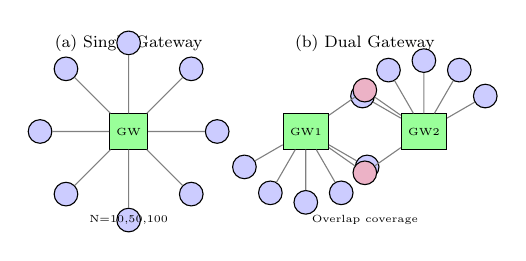
\begin{tikzpicture}[scale=0.75, transform shape,
    device/.style={circle, draw, fill=blue!20, minimum size=0.4cm, font=\tiny},
    gateway/.style={rectangle, draw, fill=green!40, minimum size=0.6cm, font=\tiny}
]
% Single Gateway (left)
\node[font=\footnotesize, align=center] at (1.5,3) {(a) Single Gateway};
\node[gateway] (gw1) at (1.5,1.5) {GW};
\foreach \i in {1,...,8} {
    \pgfmathsetmacro{\angle}{360/8*\i}
    \node[device] (d\i) at ({1.5+1.5*cos(\angle)},{1.5+1.5*sin(\angle)}) {};
    \draw[gray, thin] (gw1) -- (d\i);
}
\node[font=\tiny] at (1.5,0) {N=10,50,100};

% Dual Gateway (right)
\node[font=\footnotesize, align=center] at (5.5,3) {(b) Dual Gateway};
\node[gateway] (gw2a) at (4.5,1.5) {GW1};
\node[gateway] (gw2b) at (6.5,1.5) {GW2};
\foreach \i in {1,...,5} {
    \pgfmathsetmacro{\angle}{180+180/6*\i}
    \node[device] (e\i) at ({4.5+1.2*cos(\angle)},{1.5+1.2*sin(\angle)}) {};
    \draw[gray, thin] (gw2a) -- (e\i);
}
\foreach \i in {1,...,5} {
    \pgfmathsetmacro{\angle}{180/6*\i}
    \node[device] (f\i) at ({6.5+1.2*cos(\angle)},{1.5+1.2*sin(\angle)}) {};
    \draw[gray, thin] (gw2b) -- (f\i);
}
% Overlap zone
\node[device, fill=purple!30] (ov1) at (5.5,2.2) {};
\node[device, fill=purple!30] (ov2) at (5.5,0.8) {};
\draw[gray, thin] (gw2a) -- (ov1); \draw[gray, thin] (gw2b) -- (ov1);
\draw[gray, thin] (gw2a) -- (ov2); \draw[gray, thin] (gw2b) -- (ov2);
\node[font=\tiny] at (5.5,0) {Overlap coverage};

\end{tikzpicture}
\end{document}
